\documentclass[../norme-di-progetto.tex]{subfiles}
\begin{document}

%%%%%%%%%%%%%%%%%%%%%%%%%%%%%%%%%%%%
%%% 4.1 - GESTIONE ORGANIZZATIVA %%%
%%%%%%%%%%%%%%%%%%%%%%%%%%%%%%%%%%%%
\subsection{Gestione organizzativa}
\subsubsection{Scopo}
Questo processo ha come scopo quello di:
\begin{itemize}
  \item Creare un modello organizzativo al fine di identificare i possibili rischi;
  \item Definire un modello di sviluppo da seguire;
  \item Pianificare il lavoro al fine di rientrare nelle scadenze prefissate;
  \item Calcolare un preventivo orario per i vari ruoli e un prospetto economico per lo sviluppo del progetto;
  \item Effettuare un bilancio finale delle spese.
\end{itemize}
Queste attività sono documentate dal Responsabile nel \textsc{Piano di Progetto}.

\subsubsection{Aspettative}
Le aspettative di questo processo sono:
\begin{itemize}
  \item La corretta pianificazione delle attività da seguire;
  \item Il giusto coordinamento dei ruoli e dei compiti dei vari componenti del gruppo;
  \item La corretta gestione delle comunicazioni tra i componenti del gruppo e con il proponente;
  \item Il mantenimento del controllo sul progetto, monitorando quanto prodotto dai componenti del gruppo.
\end{itemize}

\subsubsection{Descrizione}
Le attività previste da questo processo sono contenute nel \textsc{Piano di Progetto}; queste sono:
\begin{itemize}
  \item %%% IN ATTESA DEL PdP
\end{itemize}

\subsubsection{Ruoli}
I diversi ruoli sono cambiati a rotazione fissa, in modo che ogni membro del gruppo possa ricoprire ogni ruolo almeno una volta durante il progetto. Nel \textsc{Piano di Progetto} sono pianificate e organizzate le attività assegnate ad ogni ruolo. \\
I ruoli che ogni componente del gruppo deve rappresentare sono descritti di seguito.
\paragraph{Responsabile}
Il ruolo del Responsabile è la figura cardine per quanto concerne le responsabilità di pianificazione, controllo, gestione e coordinamento di risorse all'interno del progetto. Altro compito del Responsabile è quello di fare da intermediario tra il gruppo e le persone esterne, cioè committente e proponente del capitolato. Egli, infine, è il responsabile ultimo dei risultati del progetto. \\
Nello specifico, il Responsabile:
\begin{itemize}
  \item Gestisce, coordina e controlla le risorse e le attività del gruppo;
  \item Elabora e gestisce i piani e le scadenze dei componenti del gruppo;
  \item Gestisce le criticità che emergono durante lo sviluppo del progetto;
  \item Redige il \textsc{Piano di Progetto};
  \item Approva i documenti e l'offerta proposta al committente.
\end{itemize}

\paragraph{Amministratore}
L'Amministratore è la figura che gestisce e controlla l'ambiente di lavoro. Nello specifico, l'Amministratore:
\begin{itemize}
  \item Organizza e dirige le infrastrutture di supporto;
  \item Gestisce i problemi legati alla gestione dei processi;
  \item Gestisce la documentazione del progetto;
  \item Redige le \textsc{Norme di Progetto}.
\end{itemize}

\paragraph{Analista}
L'Analista è colui che si occupa di tutte le attività di analisi. Questa figura, per sua natura, non è presente all'interno del gruppo per tutta la durata del progetto, bensì il suo ruolo si ferma all'esaurimento delle attività da lui svolte, le quali sono concentrate nella prima fase del ciclo di sviluppo. \\
Nello specifico, l'Analista:
\begin{itemize}
  \item Studia il dominio del progetto;
  \item Definisce e fissa i requisiti del progetto;
  \item Redige i documenti \textsc{Analisi dei Requisiti} e \textsc{Studio di Fattibilità}.
\end{itemize}

\paragraph{Progettista}
Il Progettista è la figura responsabile delle attività di progettazione. Nello specifico, il Progettista:
\begin{itemize}
  \item Effettuare scelte concernenti gli aspetti tecnici del progetto, basandosi sui principi di efficacia ed efficienza;
  \item Definire e sviluppare l'architettura del prodotto, sfruttando tecnologie note ed ottimizzate;
  \item Redige la Specifica Tecnica, la Definizione di Prodotto e la parte programmatica del Piano di Qualifica.
\end{itemize}

\paragraph{Programmatore}
Il Programmatore è colui che si occupa della codifica del progetto. Nello specifico, il Programmatore:
\begin{itemize}
  \item Implementa le scelte prese dal progettista e documentate nella Specifica Tecnica;
  \item Codifica e gestisce i componenti di supporto per la verifica e la validazione del codice.
\end{itemize}

\paragraph{Verificatore}
Il Verificatore è la figura che si occupa delle attività di controllo di quanto svolto dagli altri componenti del gruppo. Per fare ciò, il Verificatore deve rifarsi alle \textsc{Norme di Progetto} per controllare che quanto prodotto, sia esso documentazione o codice, segua correttamente tutte le norme documentate. Nel caso in cui trovi un errore di qualunque natura, il Verificatore non è autorizzato alla correzione di esso; deve bensì contattare colui che ha commesso il possibile errore e comunicarglielo. Sarà poi compito del redattore correggere eventualmente quanto svolto. \\
Riassumento, il Verificatore:
\begin{itemize}
  \item Ispeziona i prodotti in fase di revisione, facendo capo a quanto scritto nelle \textsc{Norme di Progetto};
  \item Evidenzia eventuali errori del prodotto ispezionato e li comunica all'autore del prodotto stesso.
\end{itemize}

\subsubsection{Procedure}
Di seguito sono riportate le procedure inerenti ai processi organizzativi che il gruppo adotterà durante l'intero ciclo di vita del prodotto.

\paragraph{Gestione delle comunicazioni}
\subparagraph{Comunicazioni Interne}
Le comunicazioni interne, cioè quelle tra i soli membri del gruppo, avvengono su tre diverse piattaforme:
\begin{itemize}
  \item Slack;
  \item Discord;
  \item Telegram.
\end{itemize}
\subparagraph*{Slack}
La piattaforma Slack viene utilizzata per le comunicazioni scritte ufficiali; è stato creato un workspace, chiamato "CoffeeCode", consistente di diversi canali:
\begin{itemize}
  \item \textbf{\#general}: canale principale, utilizzato per comunicazioni generali di natura tecnica;
  \item \textbf{\#analisi-dei-requisiti}: canale per le comunicazioni riguardanti il documento \textsc{Analisi dei Requisiti};
  \item \textbf{\#norme-di-progetto}: canale per le comunicazioni riguardanti il documento \textsc{Norme di Progetto};
  \item \textbf{\#piano-di-progetto}: canale per le comunicazioni riguardanti il documento \textsc{Piano di Progetto};
  \item \textbf{\#piano-di-qualifica}: canale per le comunicazioni riguardanti il documento \textsc{Piano di Qualifica};
  \item \textbf{\#studio-di-fattibilità}: canale per le comunicazioni riguardanti il documento \textsc{Studio di Fattibilità};
  \item \textbf{\#technology-and-tool-faq}: canale che raccoglie tutte le domande che i componenti del gruppo pongono in merito alle tecnologie utilizzate;
  \item \textbf{\#predire-in-grafana}: canale collegato alla repository Github; ogni operazione svolta sulla repository viene qui riportata dal sistema automatico "Github for Slack";
  \item \textbf{\#random}: canale riguardante le comunicazioni che non rientrano in nessuno dei precedenti argomenti.
\end{itemize}

\begin{figure}[H]
  \centering
  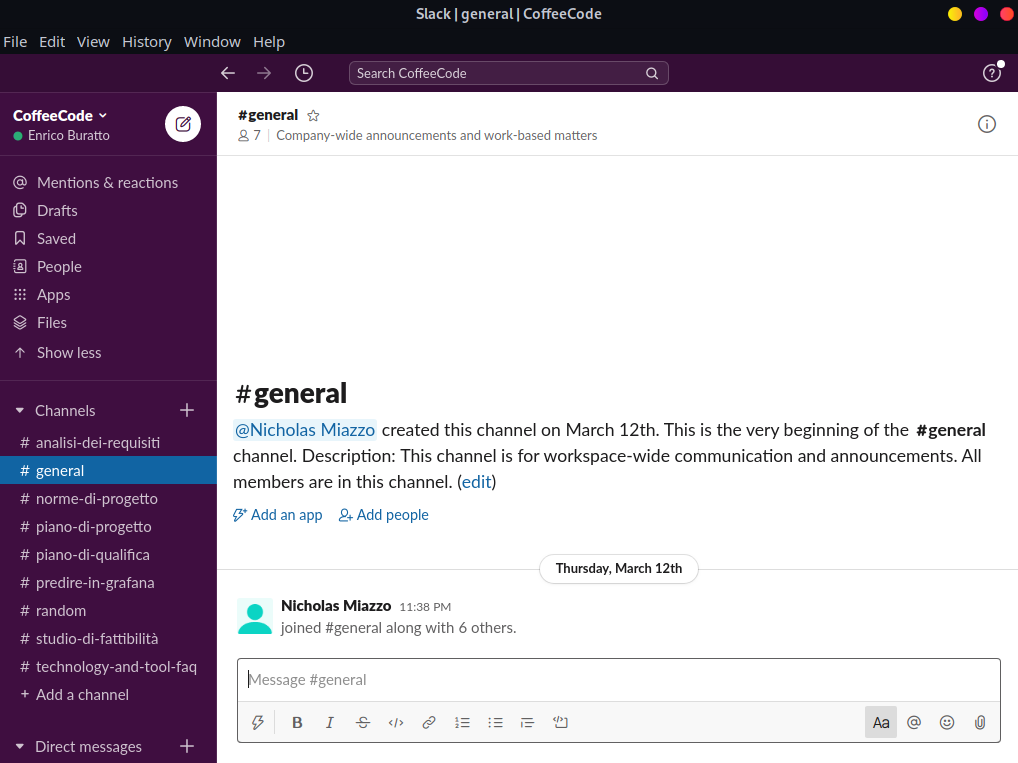
\includegraphics[width=10cm]{img/slack.png}
  \label{fig:slack}
  \caption{Slack per GNU/Linux.}
\end{figure}

\subparagraph*{Discord}
A causa dell'impossibilità di svolgere incontri \textit{vis-à-vis}, è stato deciso di utilizzare una piattaforma consona di comunicazione vocale. È quindi stato creato un server Discord, chiamato "CoffeeCode", contenente un canale \textbf{\#general} per gli incontri in tempo reale tra i componenti del gruppo.

\begin{figure}[H]
  \centering
  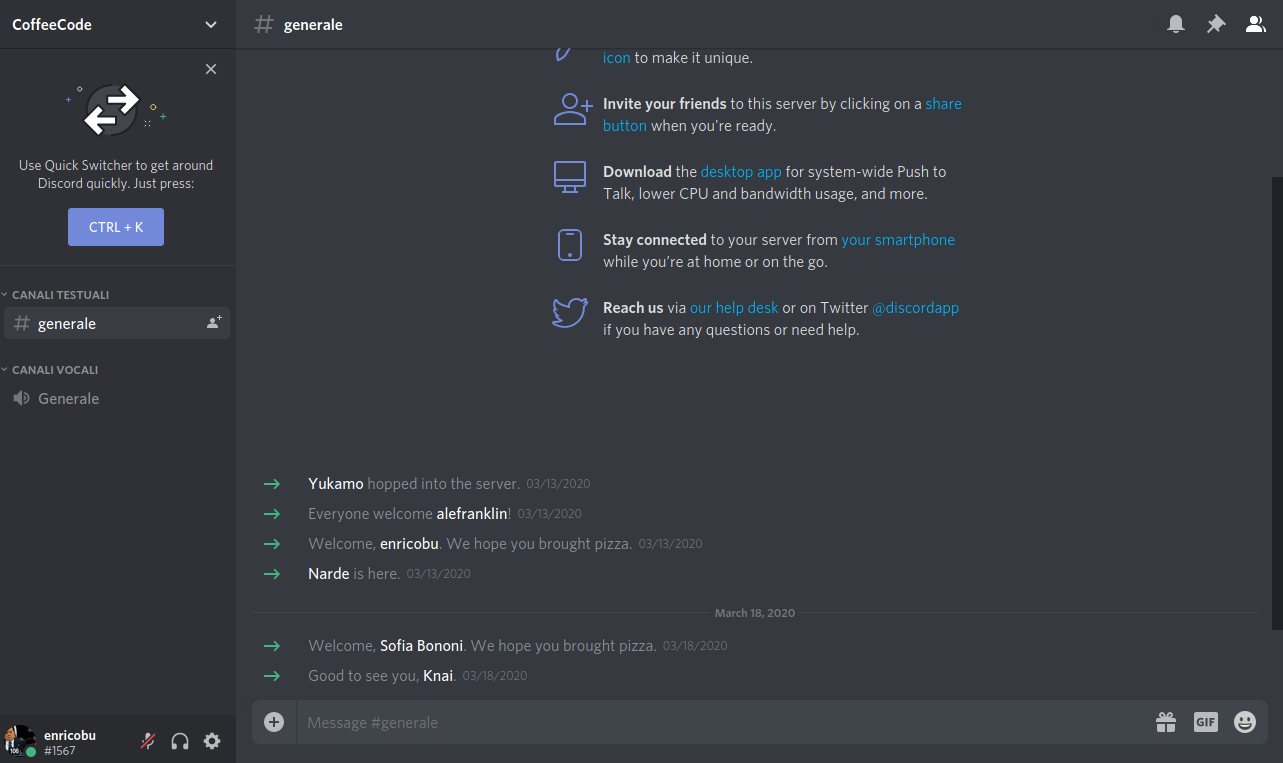
\includegraphics[width=10cm]{img/discord.png}
  \label{fig:discord}
  \caption{Discord per browser.}
\end{figure}

\subparagraph*{Telegram}
Oltre alle precedenti piattaforme, è stato creato anche un gruppo Telegram, chiamato "CoffeeCode", che il gruppo usa per le comunicazioni informali tra i componenti.

\subparagraph{Comunicazioni Esterne}
Le comunicazioni esterne riguardano i membri del gruppo, il committente e/o l'azienda proponente; queste comunicazioni sono di competenza del Responsabile. Lo strumento predefinito per le comunicazioni ufficiali è la posta elettronica, tramite l'indirizzo mail \href{coffecodeswe@gmail.com}{coffecodeswe@gmail.com}. \\
Viene inoltre utilizzata la piattaforma Skype per le comunicazioni del gruppo con l'azienda proponente, nella figura del Dr. Gregorio Piccoli.

\paragraph{Incontri}
\subparagraph{Incontri interni}
In caso se ne presenti il bisogno, il gruppo può riunirsi in via telematica attraverso la piattaforma Discord. Gli incontri interni del gruppo sono indetti dal Responsabile, in accordo con tutto il gruppo. Per fissare un appuntamento il Responsabile chiede, attraverso i già citati strumenti per le comunicazioni, la disponibilità di una data e di un orario; il gruppo conferma la disponibilità e ogni membro è tenuto ad essere presente all'orario stabilito. \\
Ogni incontro interno viene verbalizzato; a turno viene quindi individuato un segretario da parte del Responsabile, che sarà tenuto a redigere un verbale contenente le informazioni generali dell'incontro, l'ordine del giorno e le discussioni fatte tra i componenti del gruppo.

\subparagraph{Incontri esterni}
Il Responsabile, tra i cui compiti è presente anche quello di interfacciare il gruppo con i soggetti esterni, provvede a raccogliere le disponibilità dei componenti del gruppo e, successivamente, a mediare la data e l'orario con i terzi. Una volta fissato l'appuntamento, tutti i componenti del gruppo che hanno dato la disponibilità sono tenuti a presentarsi all'orario stabilito. \\
Anche in questo caso, ogni incontro viene verbalizzato; le modalità di verbalizzazione sono le stesse di quelle adottate per gli incontri interni.

\paragraph{Gestione degli strumenti di coordinamento}
L'andamento dello sviluppo viene tracciato da un Issue Tracking System. Questo permette ai membri del gruppo di avere ben chiaro, in ogni momento, quali attività sono in corso, quali sono state completate e quali saranno le prossime da svolgere. \\ L'ITS che viene utilizzato è Github Issues, il quale è persistente sulla repository stessa del progetto; da questa interfaccia il Responsabile può aprire nuove \textit{issues}, includendo una descrizione di ciò che deve essere fatto e assegnandole a specifici membri del gruppo.

\begin{figure}[H]
  \centering
  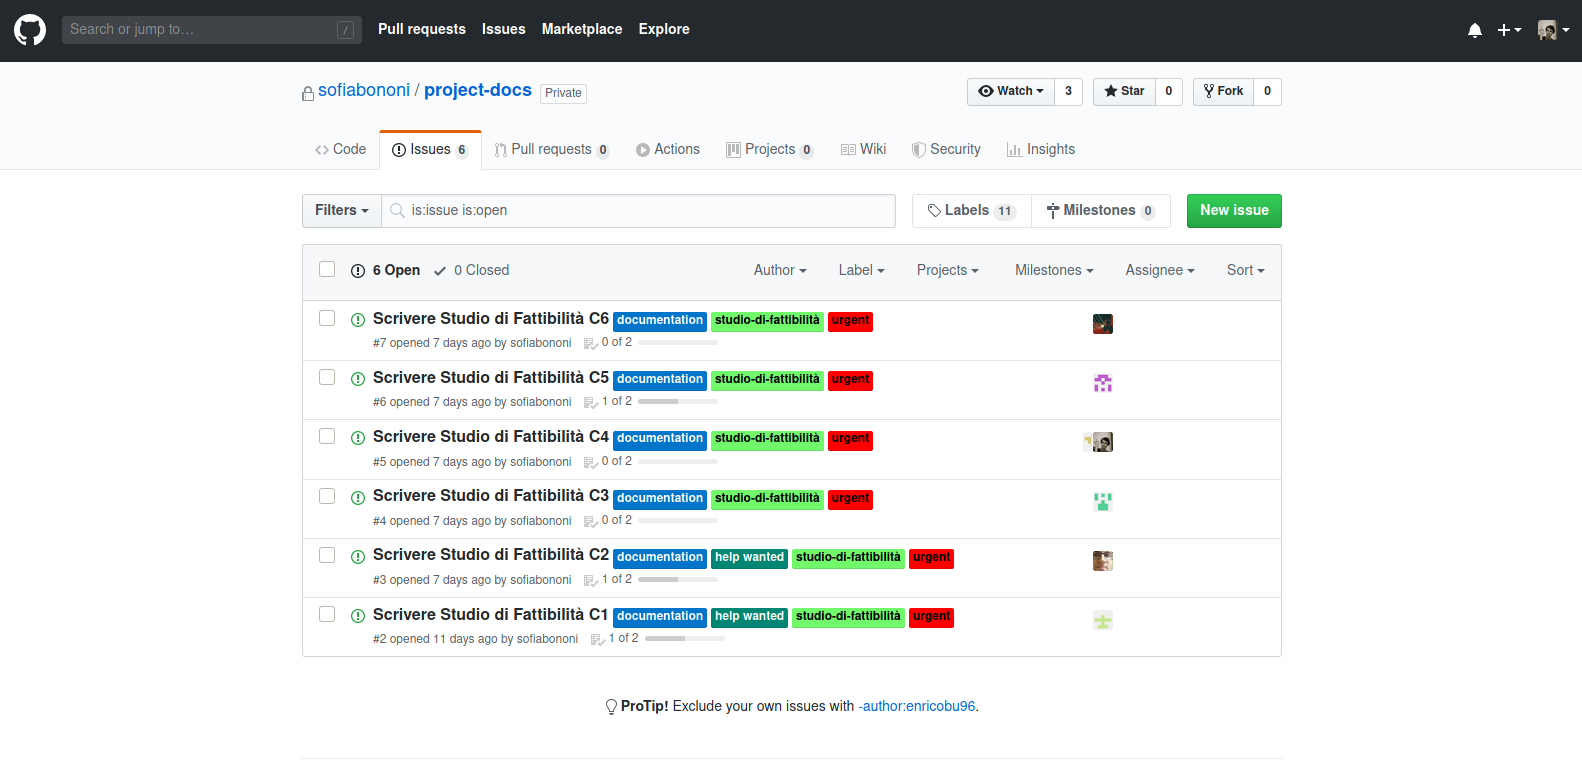
\includegraphics[width=10cm]{img/issues.png}
  \label{fig:sheets}
  \caption{Github Issues.}
\end{figure}

\paragraph{Gestione dei rischi}
I rischi vengono rilevati dal Responsabile e da lui riportati nel \textsc{Piano di Progetto}; è una procedura dinamica: nel caso in cui vengano rilevati nuovi rischi, questi saranno aggiunti nell'analisi dei rischi. La procedura che il Responsabile dovrà seguire per la gestione dei rischi è la seguente:
\begin{itemize}
  \item Individuare i nuovi rischi e monitorare quelli già previsti;
  \item Registrare ogni riscontro previsto dei rischi nel \textsc{Piano di Progetto};
  \item Aggiungere i nuovi rischi che vengono man mano individuati nel \textsc{Piano di Progetto};
  \item Ridefinire, nel caso in cui si rendesse necessario, le strategie per la gestione dei rischi.
\end{itemize}
\subparagraph*{Codifica}
La codifica dei rischi è così definita: %%% DA DISCUTERNE %%%
\begin{itemize}
  \item \textbf{RT}: Rischi Tecnologici;
  \item \textbf{RO}: Rischi Organizzativi;
  \item \textbf{RI}: Rischi Interpersonali.
\end{itemize}

\subsubsection{Strumenti}
Per tutta la durata del progetto, il gruppo si servirà di svariati strumenti per organizzare, gestire e svolgere le varie attività.
\subparagraph{Visual Studio Code}
Lo sviluppo dell'intero prodotto è eseguito nell'\glossario{IDE} Visual Studio Code, con l'aggiunta delle seguenti estensioni:
\begin{itemize}
  \item \textbf{Git Graph}: permette di utilizzare azioni Git a partire dal grafo della \glossario{repository};
  \item \textbf{LaTeX Workshop}: fornisce tutte le feature necessarie a scrittura, anteprima e compilazione di documenti \LaTeX;
  \item \textbf{GitHub Pull Requests}: permette di revisionare e gestire le Pull Requests di Github;
  \item \textbf{GitLens}: permette di visualizzare la paternità di ogni porzione di codice all'interno dell'editor;
  \item \textbf{Spell Right}: \glossario{spellchecker} multilingue e offline, permette il controllo grammaticale di quanto scritto;
  \item \textbf{Todo Tree}: permette la redazione di \glossario{TODO lists};
  \item \textbf{Prettier - Code formatter}: formatta il codice in maniera più leggibile e più immediata;
  \item \textbf{PowerShell}: solo per utenti Windows; permette di sviluppare codice in linguaggio PowerShell.
\end{itemize}

\begin{figure}[H]
  \centering
  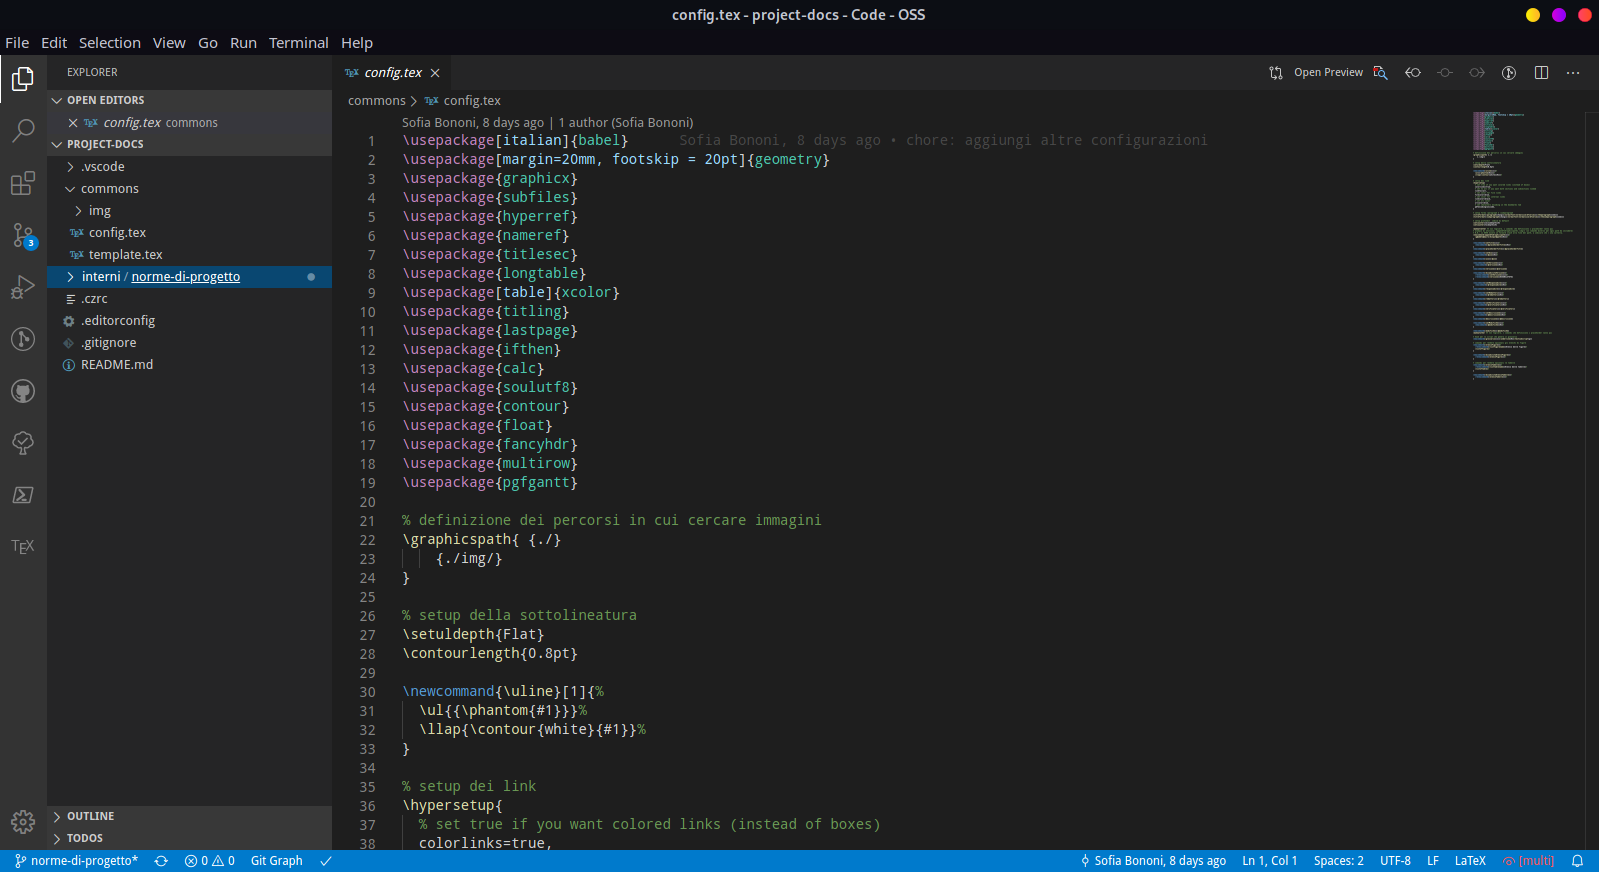
\includegraphics[width=10cm]{img/vscode.png}
  \label{fig:github}
  \caption{Visual Studio Code per GNU/Linux.}
\end{figure}

\subparagraph{GanttProject}
GanttProject è un software di \textit{project management} che permette di progettare lo \textit{scheduling} di tasks e organizzare le risorse con l'ausilio di grafici. Questo strumento è stato utilizzato principalmente per costruire i diagrammi di Gantt presenti nel \textsc{Piano di Progetto}.

\begin{figure}[H]
  \centering
  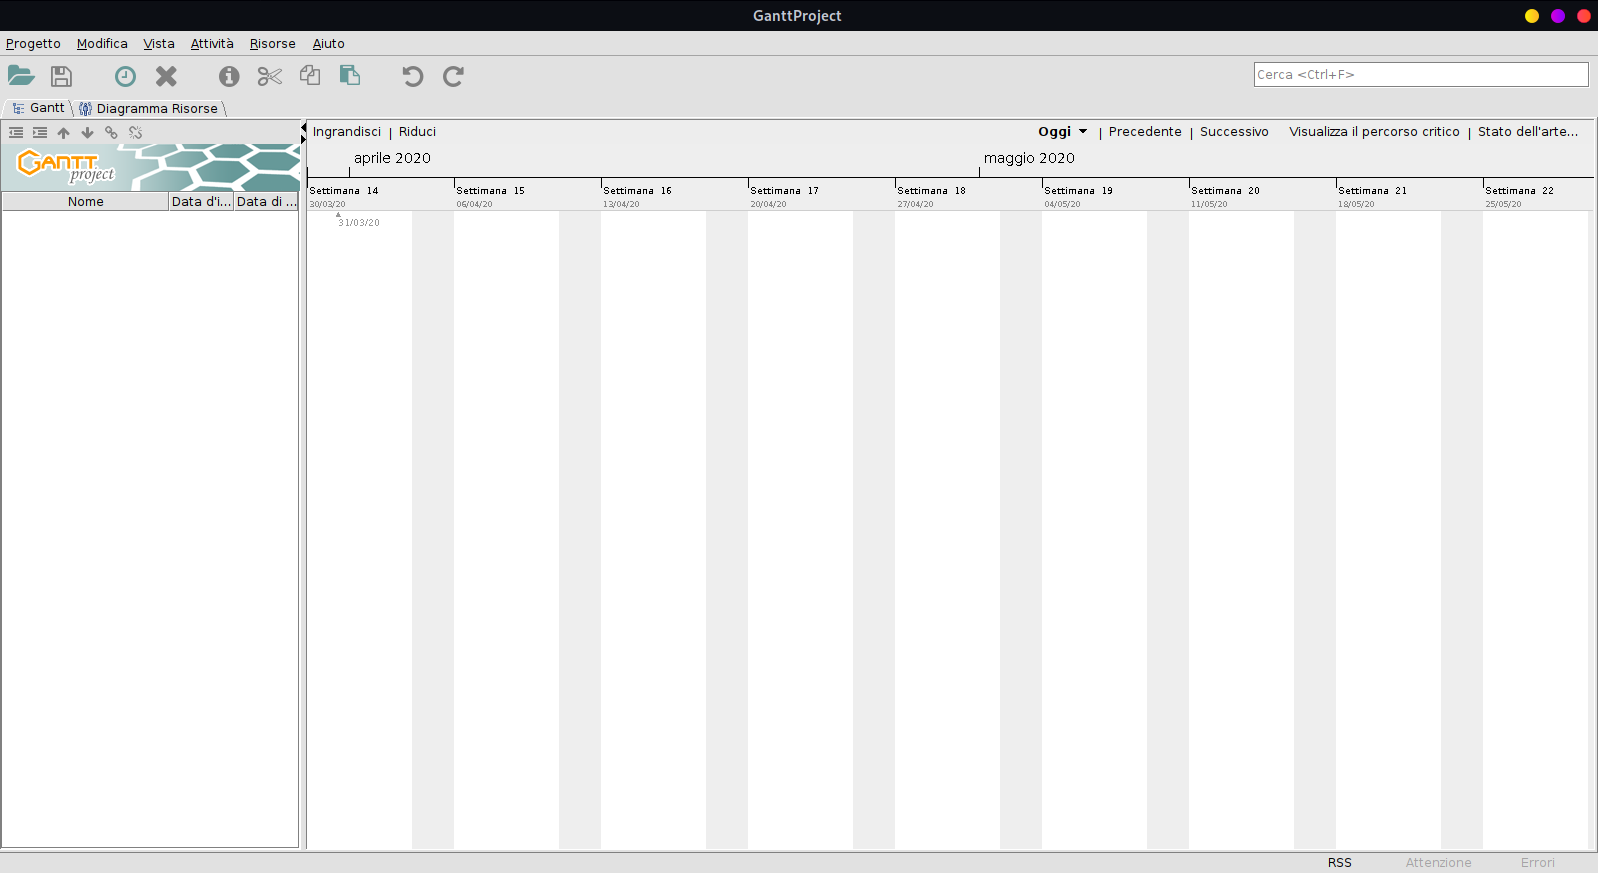
\includegraphics[width=10cm]{img/gantt.png}
  \label{fig:gantt}
  \caption{GanttProject per GNU/Linux.}
\end{figure}

\subparagraph{Google Sheets}
Google Sheets è un programma, appartenente alla \textit{suite office} di Google, per la creazione di fogli di calcolo. Questo applicativo è stato usato dal gruppo per la creazione delle tabelle e dei grafici presenti nel \textsc{Piano di Progetto}.

\begin{figure}[H]
  \centering
  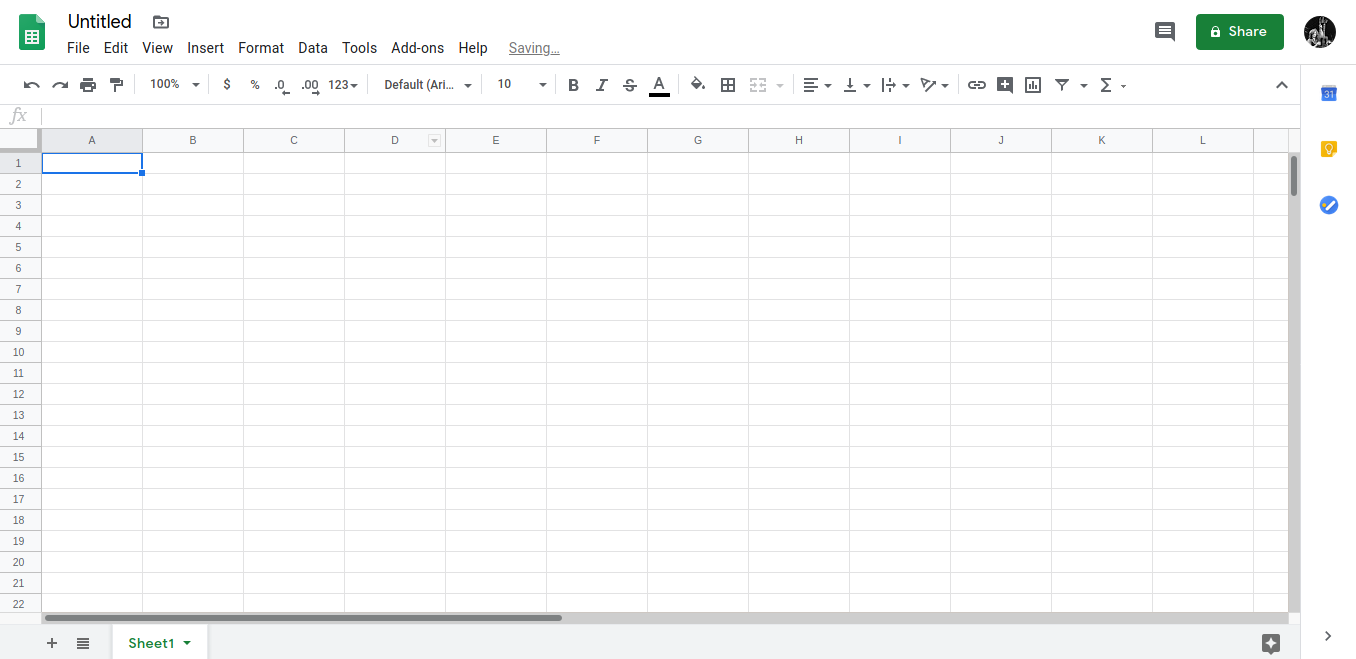
\includegraphics[width=10cm]{img/sheets.png}
  \label{fig:sheets}
  \caption{Piattaforma online \href{https://docs.google.com/spreadsheets/u/0/}{Google Sheets}.}
\end{figure}

\subparagraph{Altri strumenti}
Gli altri strumenti di cui il gruppo fa uso, già documentati nelle \textsc{Norme di Progetto}, sono:
\begin{itemize}
  \item Telegram;
  \item Git;
  \item Git Commitizen;
  \item Github;
  \item Google Drive;
  \item Skype;
  \item Microsoft Teams.
\end{itemize}

\paragraph{Sistemi Operativi}
Ogni strumento utilizzato dal gruppo è compatibile con ogni piattaforma; i Sistemi Operativi usati dai componenti del gruppo possono essere perciò diversi. I sistemi utilizzati sono:
\begin{itemize}
  \item Windows 10;
  \item macOS Catalina;
  \item Ubuntu 19.10;
  \item Debian 10;
  \item Manjaro Linux.
\end{itemize}

%%%%%%%%%%%%%%%%%%%%%%%%
%%% 4.2 - FORMAZIONE %%%
%%%%%%%%%%%%%%%%%%%%%%%%
\subsubsection{Formazione}
\paragraph{Scopo}
I membri del gruppo sono tenuti ad essere formati sui diversi ambiti su cui verte il progetto, dalle tecnologie necessarie allo sviluppo del software ai diversi strumenti organizzativi e di supporto normati da questo documento. \\
\paragraph{Piano di formazione}
La formazione avviene in due diverse modalità:
\begin{itemize}
  \item Tramite erogazione di brevi seminari sulle tecnologie da parte dell'azienda;
  \item Tramite auto-apprendimento, studiando cioè la documentazione necessaria individualmente.
\end{itemize}
I brevi seminari erogati dall'azienda coprono buona parte delle conoscenze di Machine Learning necessarie allo sviluppo del software. \\ Per la formazione individuale, i membri del gruppo devono fare riferimento alla seguente documentazione:
\begin{itemize}
  \item \textbf{Javascript}: \href{https://devdocs.io/javascript/}{https://devdocs.io/javascript/};
  \item \textbf{Grafana}: \href{https://grafana.com/docs/grafana/latest/}{https://grafana.com/docs/grafana/latest/};
  \item \textbf{Electron}: \href{https://www.electronjs.org/docs}{https://www.electronjs.org/docs};
  \item \textbf{\LaTeX}: \href{https://www.latex-project.org/help/documentation/}{https://www.latex-project.org/help/documentation/};
  \item \textbf{Git}: \href{https://git-scm.com/doc}{https://git-scm.com/doc};
  \item \textbf{Github}: \href{https://help.github.com/en}{https://help.github.com/en};
  \item \textbf{Git Commitizen}: \href{http://commitizen.github.io/cz-cli/}{http://commitizen.github.io/cz-cli/}.
\end{itemize}
\end{document}
